Kapitola výsledky je rozdělena na čtyři části. První dvě kapitoly prezentují
realizované softwarové řešení pro online a offline hodnocení srdeční aktivity.
Následně sekce~\ref{sections:results_probands} uvádí výsledky analýzy
zpracovaných záznamů a statistického testování normality sledovaných veličin
(viz kapitola~\ref{section:selected_stats_vals}).
Sekce~\ref{sections:results_analysis} popisuje výsledky statistického ověření
metody Poincarého grafu v rámci hodnocení HRV u zpracovaných EKG záznamů.

\subsection{Softwarové řešení pro offline hodnocení EKG}
\label{sections:results_online}
Výstup jednotlivých fází zpracování EKG záznamů (viz kapitola
\ref{section:offline_processing}) byl sjednocen do jednoho hlavního okna pomocí
integrovaného \textit{App Designeru} \cite{matlabAPPDESIGNER} v programovém
prostředí \textit{MATLAB}. Výsledkem je spustitelná interaktivní aplikace. Po
spuštění aplikace lze v menu pomocí tlačítka \textbf{Load signal} nahrát EKG
signál ve formátu CSV nebo MAT. Po výběru EKG signálu je uživatel tázán aby
zadal vzorkovací frekvenci signálu. EKG signál je následně adaptivně zpracován.
\begin{figure}[h]
	\begin{center}
		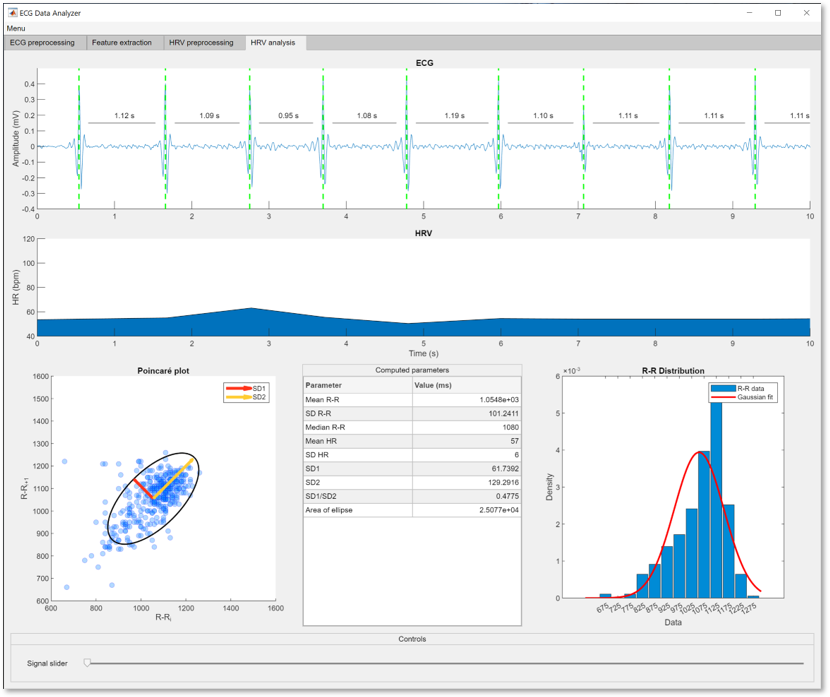
\includegraphics[width=1\textwidth]{../assets/matlab_EDA/tab4}
		\caption{Hlavní okno aplikace -- karta \textbf{HRV analysis}}
		\label{fig:results_matlab_tab4}
	\end{center}
\end{figure}
Na Obr.~\ref{fig:results_matlab_tab4} lze vidět otevřenou kartu \textbf{HRV
analysis}, která vizualizuje výstup HRV analýzy vycházející ze všech předešlých
fází zpracování. Všechny karty aplikace jsou uvedené v Příloze B. Jednotlivé
karty jsou mezi sebou propojené. Pokud například uživatel v jedné kartě posune
signál na určitý čas, tak se tato změna aplikuje na signály ostatních karet.

% \begin{figure}[h]
% 	\begin{center}
% 		\textcolor{cyan}{\fboxrule=0.5pt\fboxsep=0pt\fbox{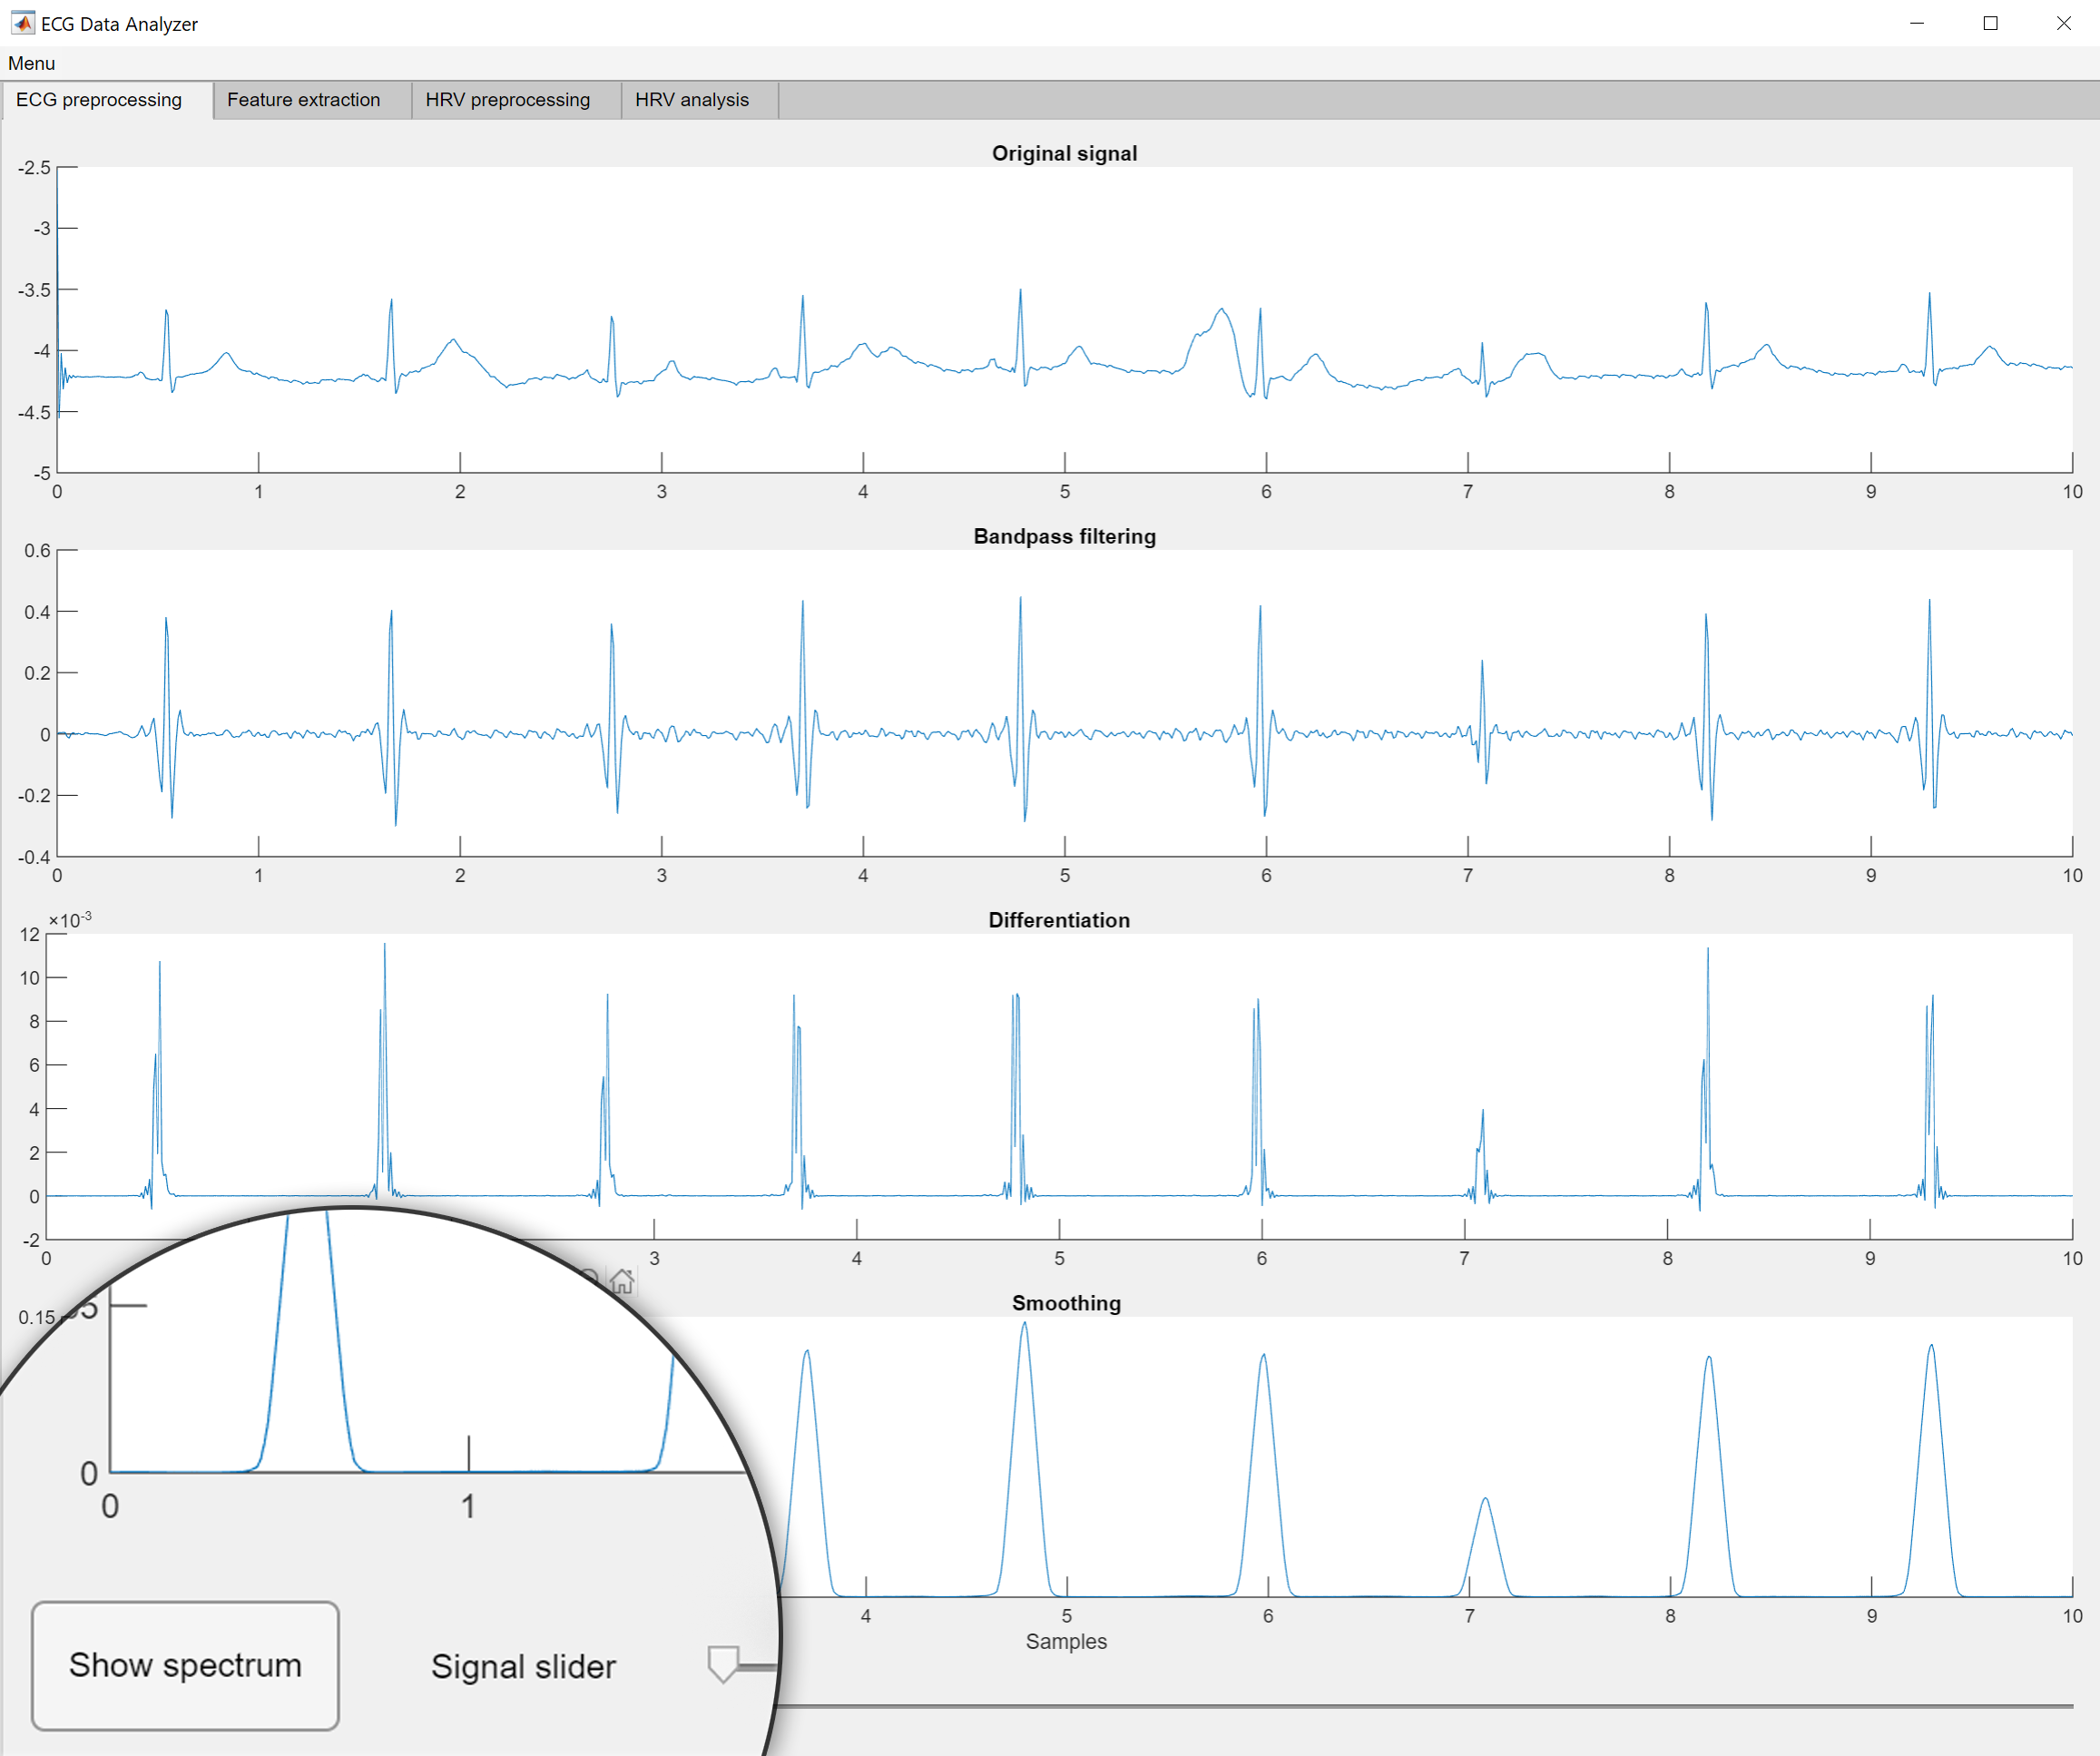
\includegraphics[width=1\textwidth]{../assets/matlab_EDA/tab1}}}
% 		\caption{Hlavní okno aplikace -- karta ECG preprocessing}
% 		\label{fig:results_matlab_tab1}
% 	\end{center}
% \end{figure}

% \begin{figure}[h]
% 	\begin{center}
% 		\textcolor{cyan}{\fboxrule=0.5pt\fboxsep=0pt\fbox{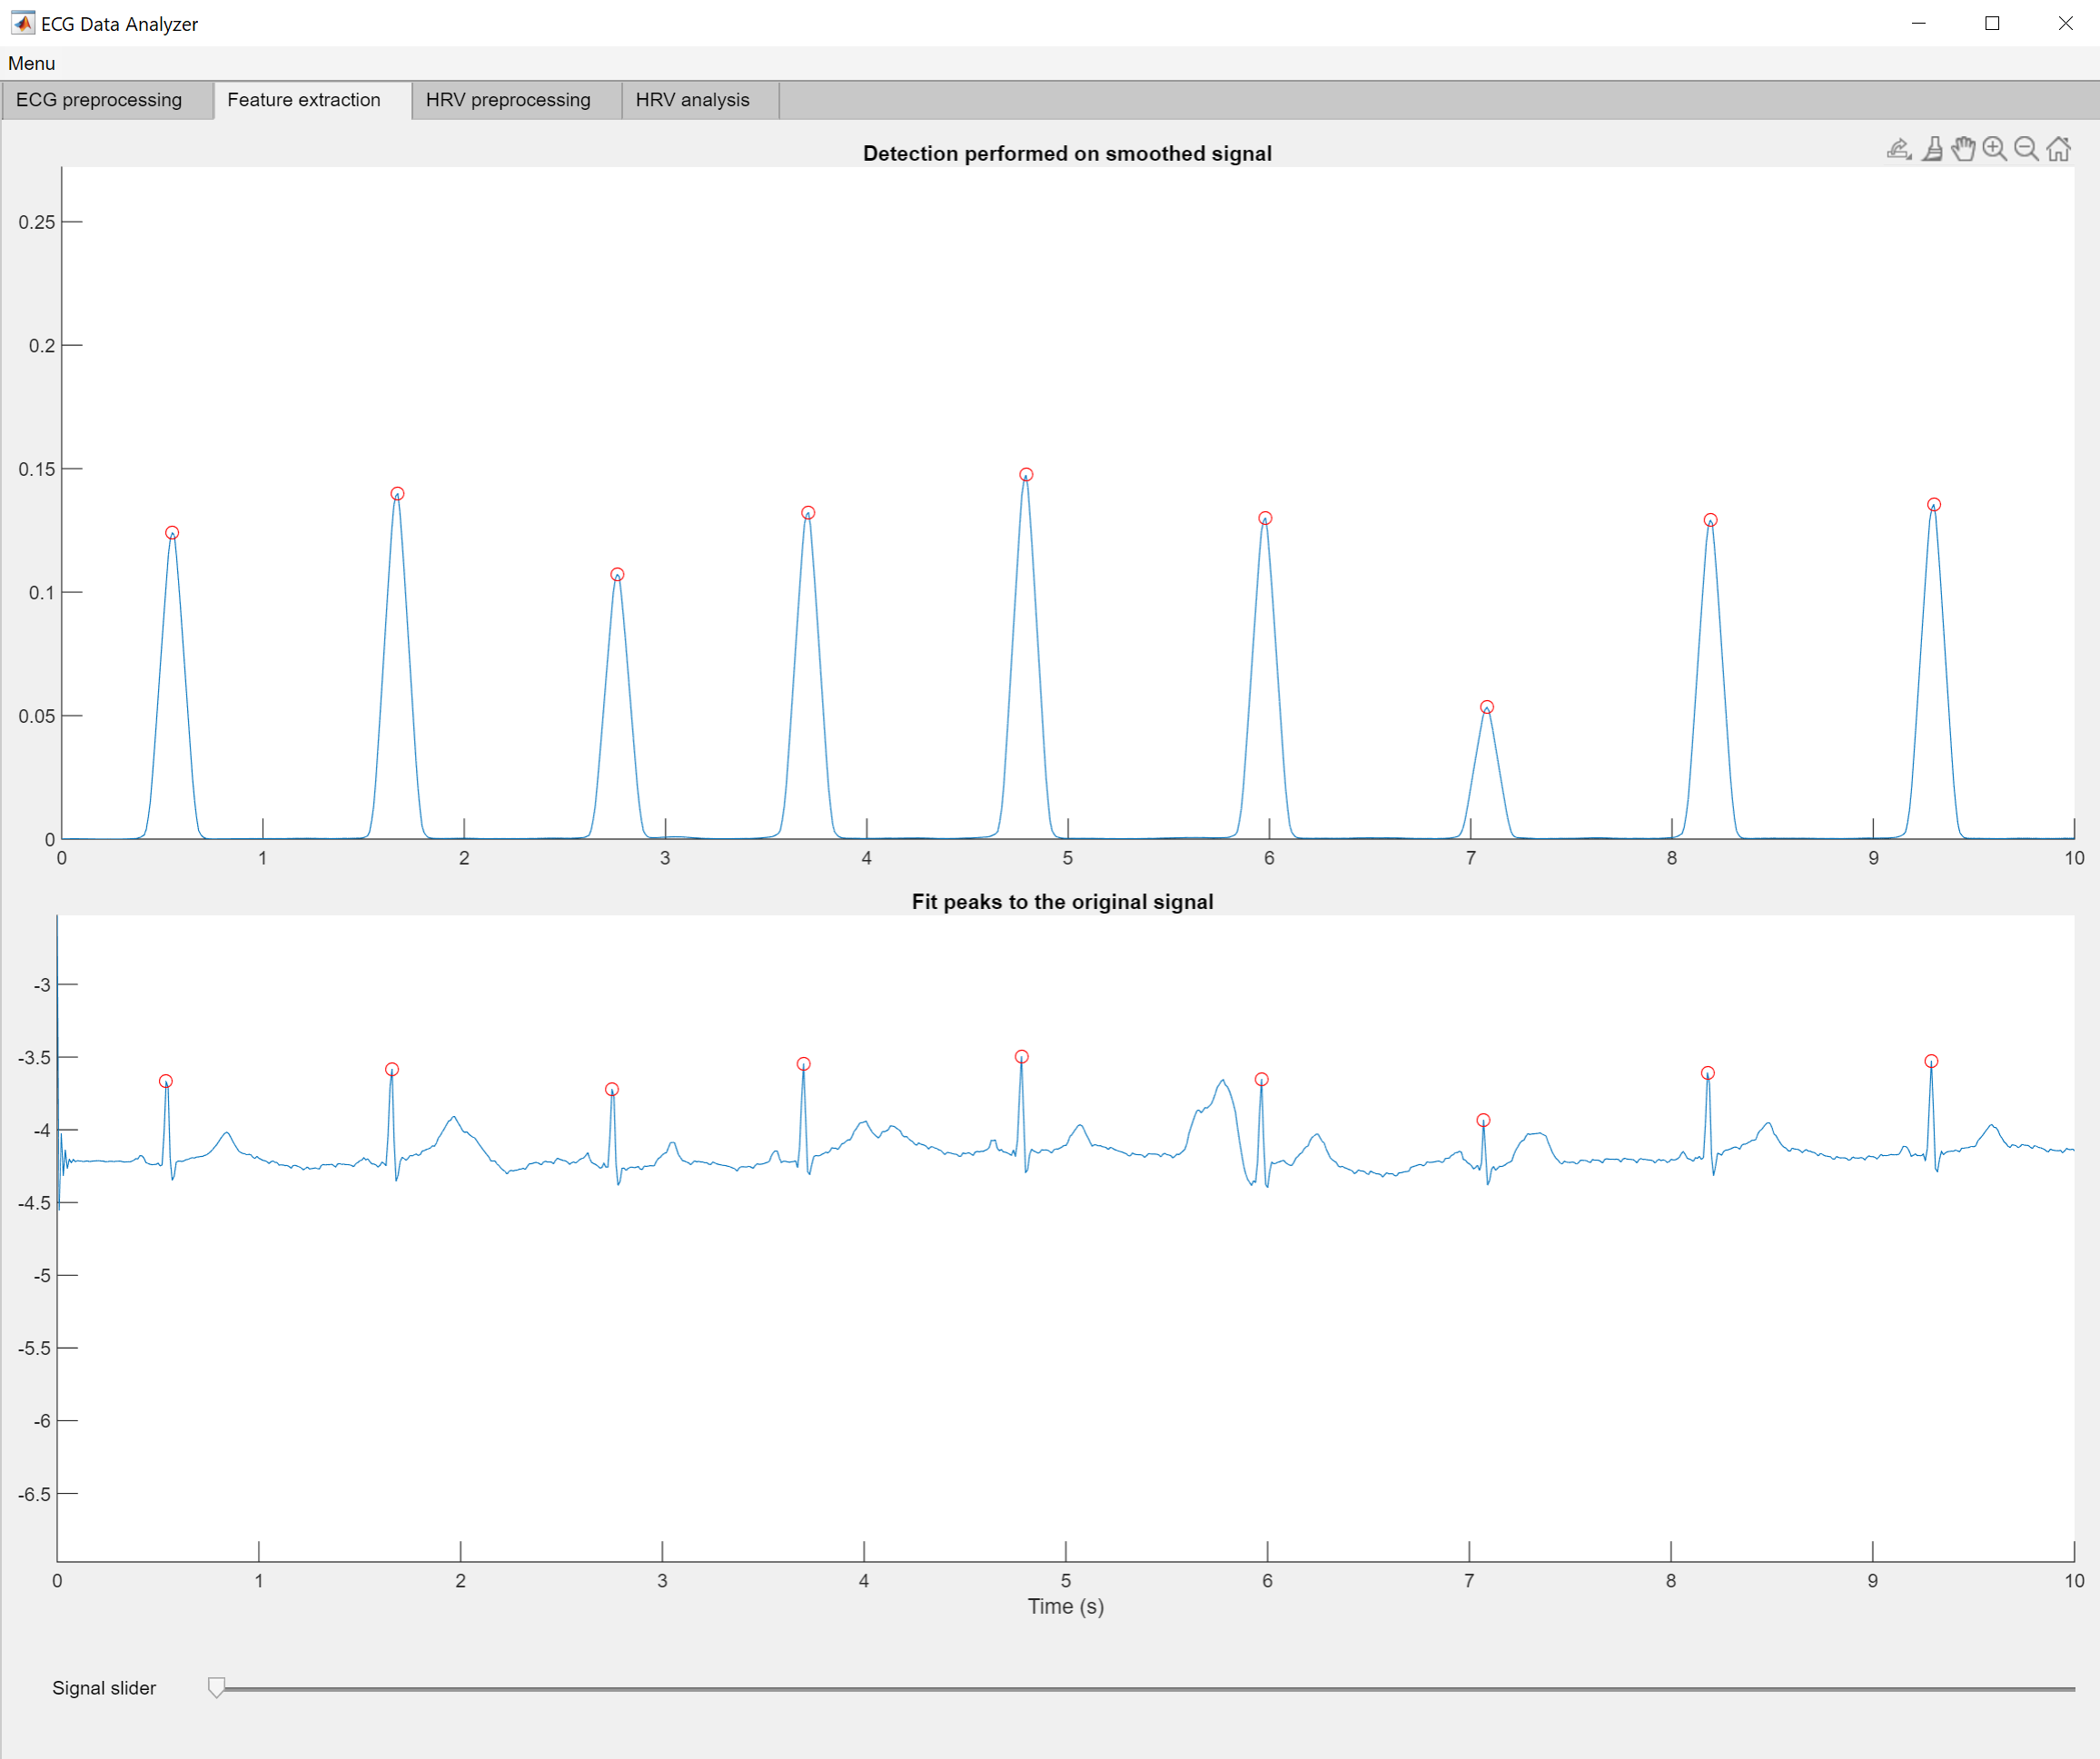
\includegraphics[width=1\textwidth]{../assets/matlab_EDA/tab2}}}
% 		\caption{Hlavní okno aplikace -- karta Feature extraction}
% 		\label{fig:results_matlab_tab2}
% 	\end{center}
% \end{figure}

% \begin{figure}[h]
% 	\begin{center}
% 		\textcolor{cyan}{\fboxrule=0.5pt\fboxsep=0pt\fbox{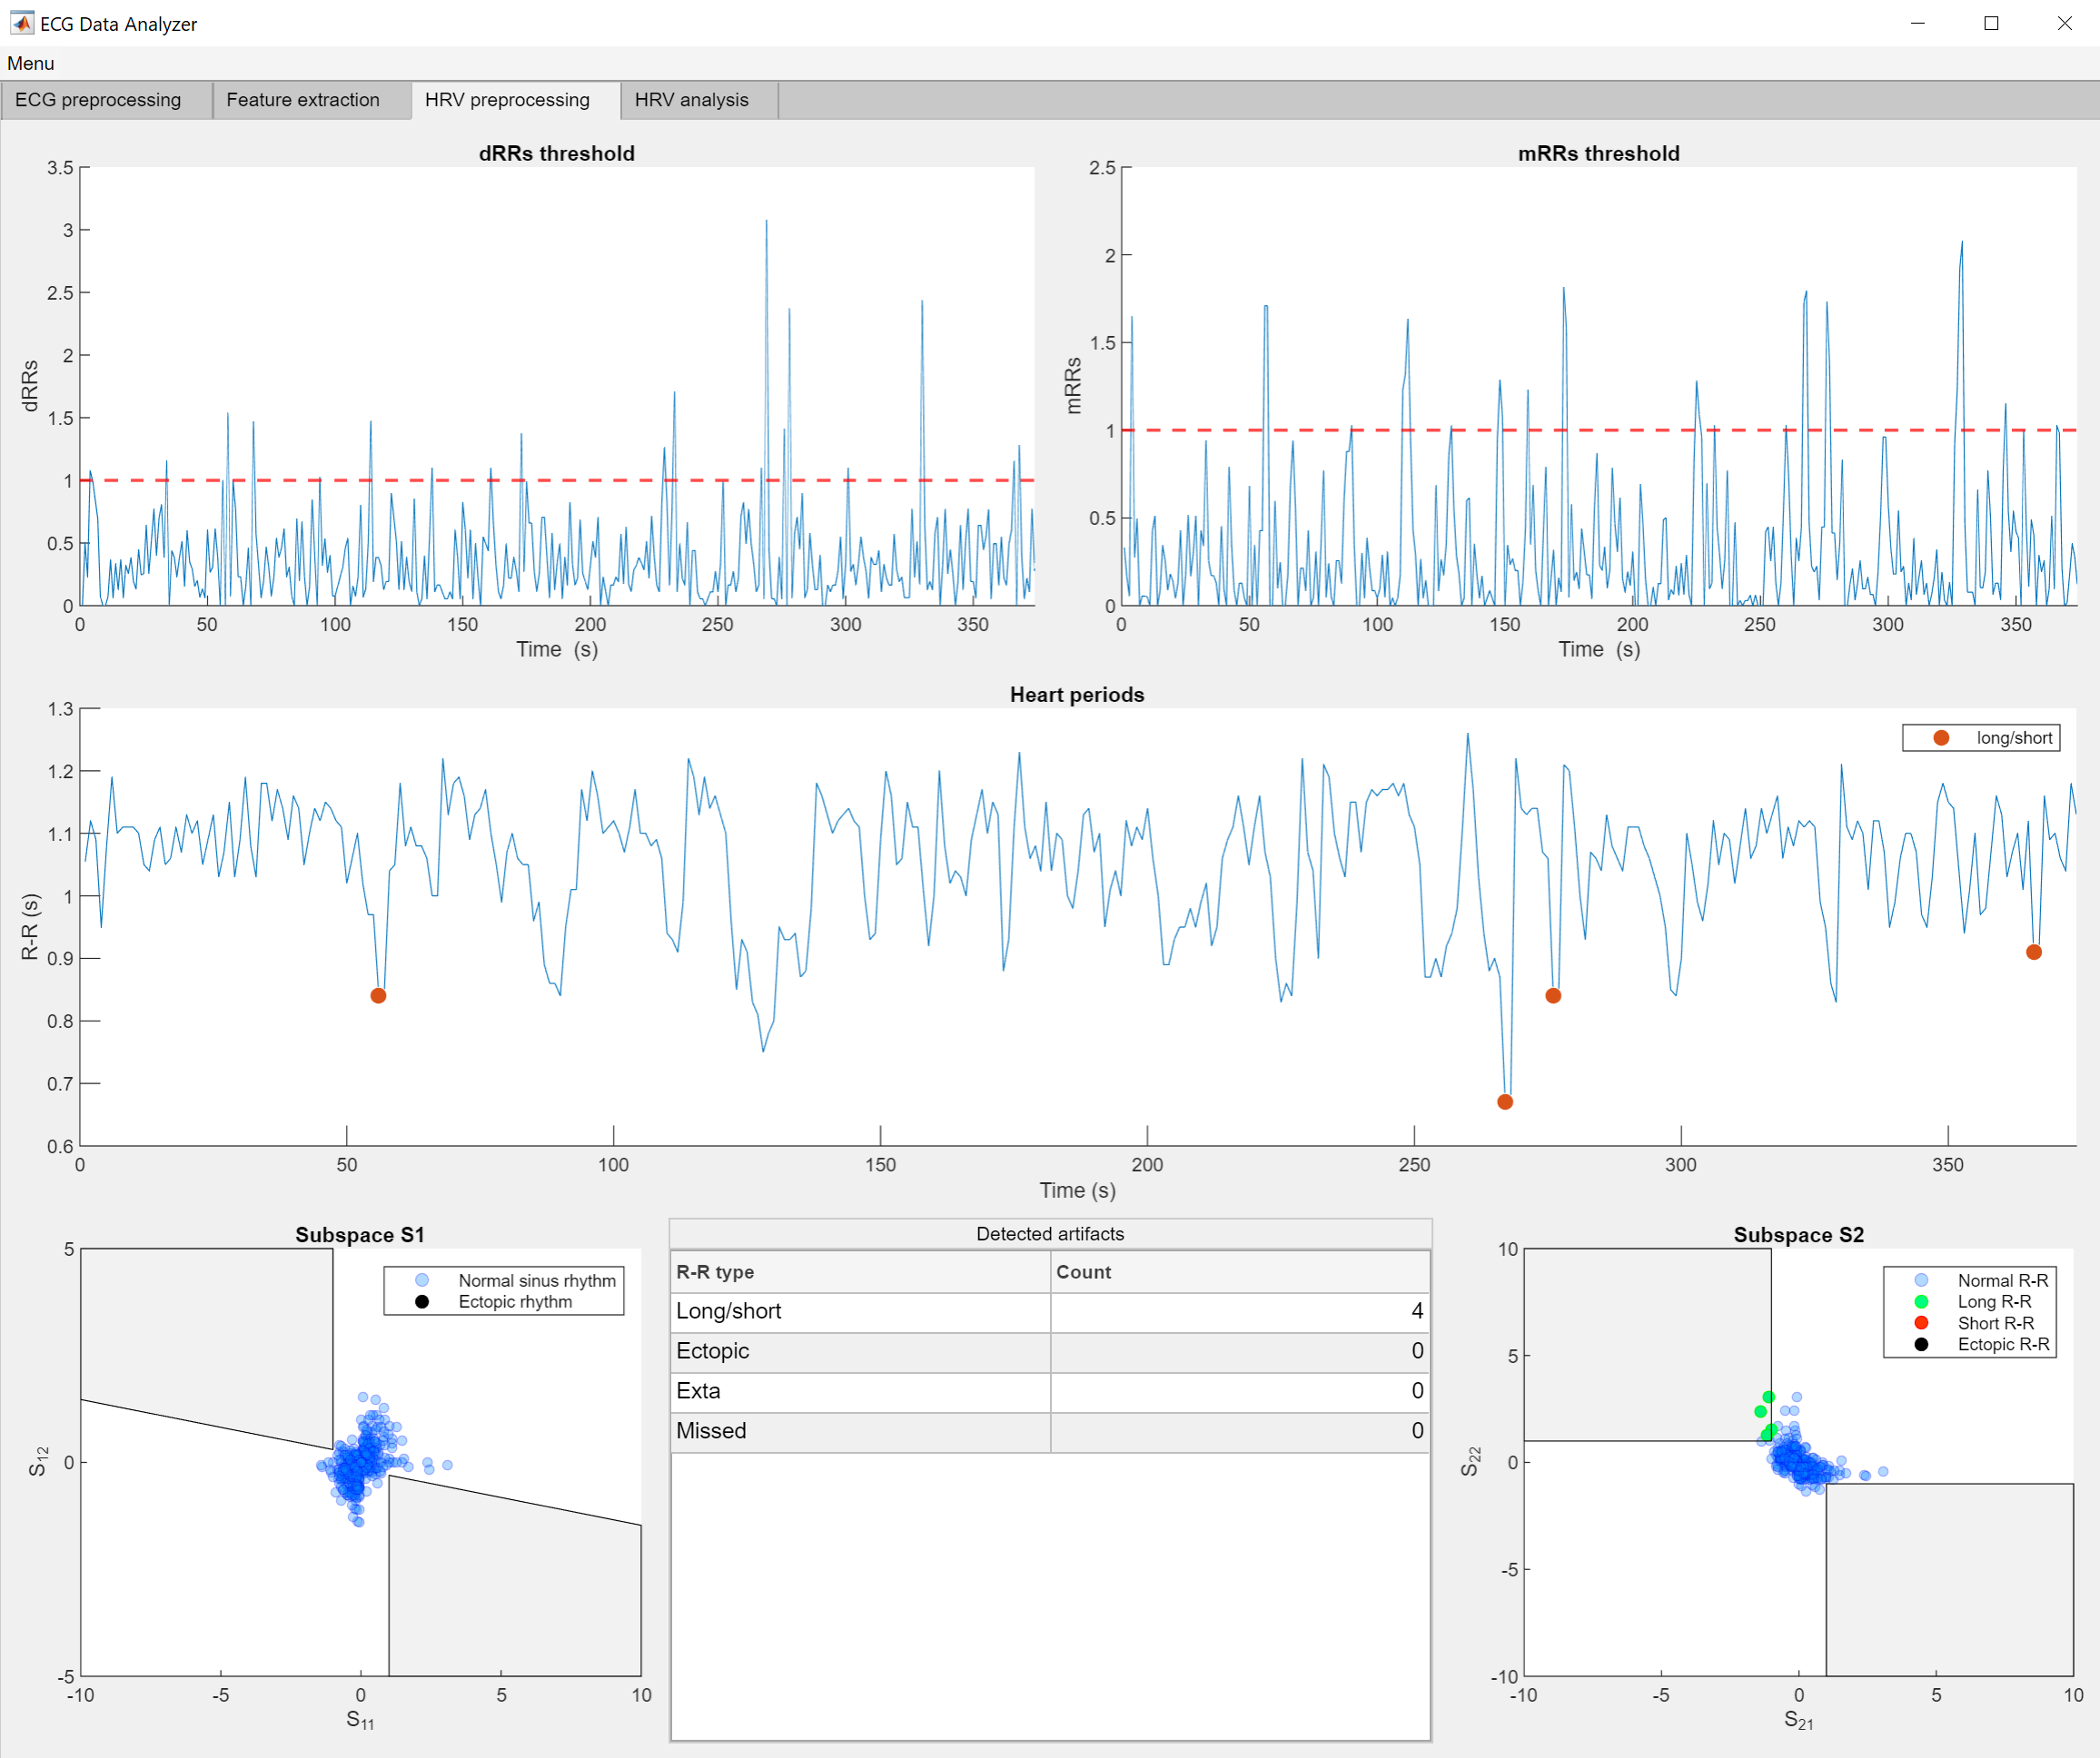
\includegraphics[width=1\textwidth]{../assets/matlab_EDA/tab3}}}
% 		\caption{Hlavní okno aplikace -- HRV preprocessing}
% 		\label{fig:results_matlab_tab3}
% 	\end{center}
% \end{figure}


\subsection{Softwarové řešení pro online hodnocení EKG}
\label{sections:result_offline}
Pro účely online analýzy EKG a sběr dat byla naprogramovaná aplikace jménem
\textit{BBPM} v prostředí \textit{Python}. Prostředí \textit{Python} bylo
zvoleno na základě jeho open-source licence, která jej umožňuje zdarma používat
a volně nebo i komerčně distribuovat vyvinutá řešení. Aplikaci lze vidět na
Obr.~\ref{fig:results_bbpm}. Realizované řešení bylo použito pro pilotní měření
a záznam surových EKG signálů u kontrolní skupiny probandů (viz
kapitola~\ref{section:probands}). Aplikace je detailněji popsaná v
kapitole~\ref{section:online_processing}.

\begin{figure}[H]
	\begin{center}
		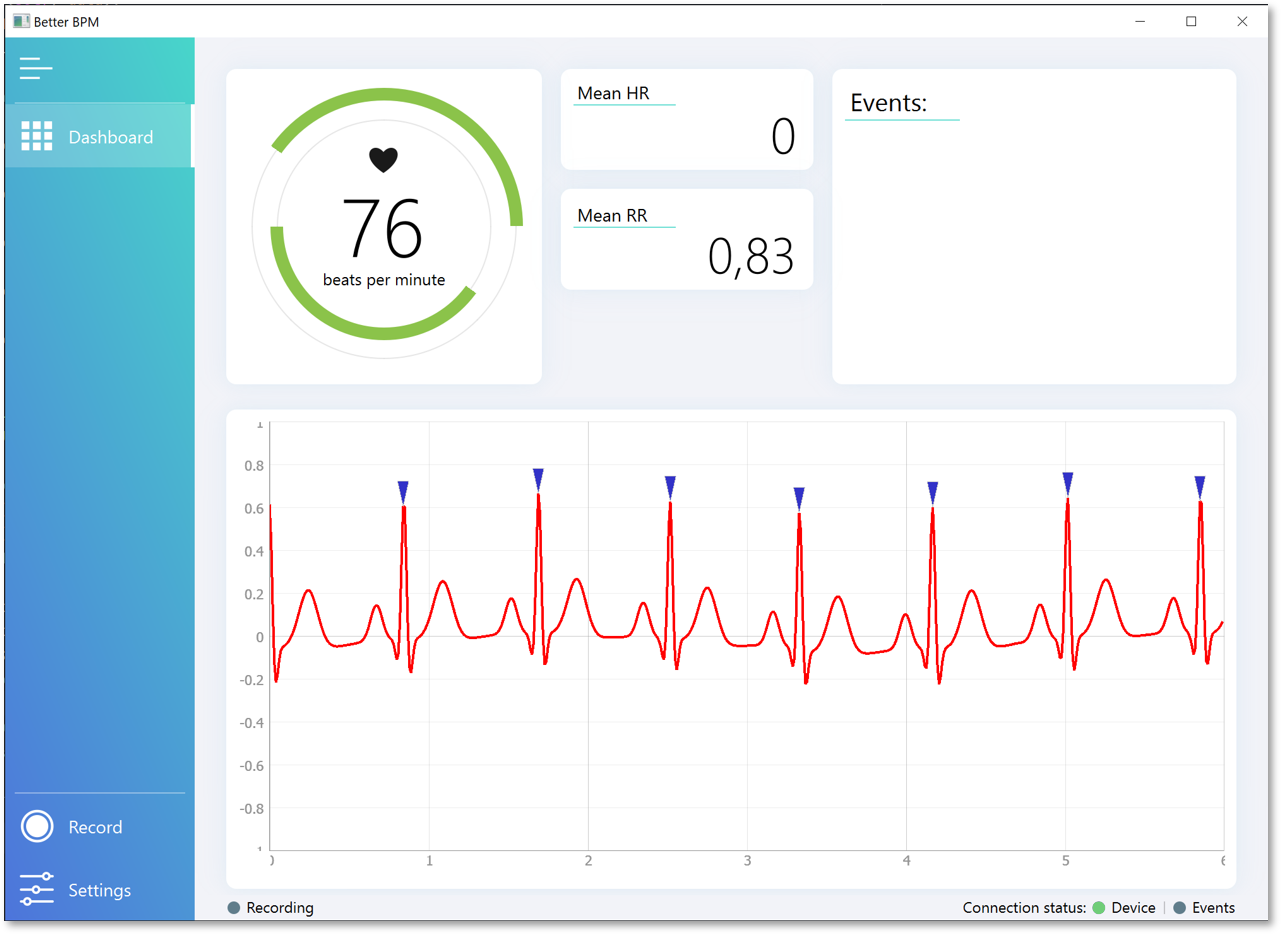
\includegraphics[width=1\textwidth]{../assets/bbpm/bbpm_app}
		\caption{Aplikace \textit{BBPM}}
		\label{fig:results_bbpm}
	\end{center}
\end{figure}

\clearpage

\subsection{Kontrolní skupina}
\label{sections:results_probands}
V rámci kontrolní skupiny (viz sekce~\ref{section:probands}) bylo dle postupu v
kapitole~\ref{section:measurement_methodology} naměřeno 5 EKG záznamů aplikací
\textit{BBPM} (\ref{section:online_processing}). Záznamy byly následně
zpracované realizovaným SW řešením popsaným v
sekci~\ref{section:offline_processing}. V následujících podkapitolách jsou
prezentovány výsledky jednotlivých fází zpracování realizovaného offline řešení
pro hodnocení EKG.

\subsubsection{Detekované R vlny}
Následující tabulka \ref{tab:detected_artifacts} uvádí výstup fáze zpracování
detekovaných komponentů společně s vypočítanými parametry: průměrná hodnota
korigovaných (normálních, N-N) R-R intervalů (mNN), průměrná hodnota srdeční
frekvence (mHR), směrodatná odchylka R-R intervalů (SDNN) a směrodatná odchylka
srdeční frekvence (SDHR). Hodnoty parametrů vychází z R vln, který byly
korigovány algoritmem popsaným v sekci~\ref{section:measurement_process}. Z
korigovaných veličin vychází následná HRV analýza. Detekované artefakty uvádí
tabulka~\ref{tab:detected_artifacts} v následující sekci.

\begin{table}[h]
	\captionsetup{font=small,skip=0.5pt}
	\catcode`\-=12
	\begin{center}
		\caption{\label{tab:corrected_components} Korigované R vlny s vypočítanými parametry časové série R-R intervalů z klidové částí měření (N) a při Stroopově testu (S)}
		\vspace{1ex}
		\setlength{\tabcolsep}{13pt}
		\renewcommand{\arraystretch}{1.3}
		\begin{tabular}{llccccc}
			\noalign{\hrule height 2pt}
			                    &   &                      & \multicolumn{4}{c}{\textbf{Vypočítané parametry (ms)}}                                                 \\	\cline{4-7}
			                    &   &                      & \textbf{mNN}                                           & \textbf{mHR}  & \textbf{SDNN} & \textbf{SDHR} \\
			                    &   & \textbf{Počet R vln} & \small{(ms)}                                           & \small{(bpm)} & \small{(ms)}  & \small{(bpm)} \\	\noalign{\hrule height 2pt}
			\textbf{1. proband} & N & 369                  & 957                                                    & 64            & 139           & 10            \\
			                    & S & 428                  & 1043                                                   & 58            & 114           & 7             \\	\noalign{\hrule}
			\textbf{2. proband} & N & 374                  & 1055                                                   & 57            & 101           & 6             \\
			                    & S & 270                  & 982                                                    & 62            & 81            & 5             \\	\noalign{\hrule}
			\textbf{3. proband} & N & 535                  & 635                                                    & 95            & 49            & 7             \\
			                    & S & 542                  & 586                                                    & 103           & 52            & 9             \\	\noalign{\hrule}
			\textbf{4. proband} & N & 539                  & 649                                                    & 93            & 56            & 8             \\
			                    & S & 607                  & 536                                                    & 113           & 47            & 10            \\	\noalign{\hrule}
			\textbf{5. proband} & N & 447                  & 920                                                    & 67            & 142           & 10            \\
			                    & S & 321                  & 897                                                    & 68            & 91            & 7             \\ 	\noalign{\hrule height 2pt}
		\end{tabular}
	\end{center}
\end{table}

\subsubsection{Detekované artefakty R-R intervalů}
Včetně korigovaných R vln jsou výstupními parametry fáze zpracování detekovaných
komponentů také detekované artefakty v rámci R-R intervalů. Počty detekovaných
artefaktů za celý 10 minutový EKG záznam jsou pro každého probanda vyneseny v
tabulce~\ref{tab:detected_artifacts}. Detekce artefaktů, společně se způsoby
korekce jejich jednotlivých typů, je popsaná v
sekci~\ref{section:components_processing}.

\begin{table}[h]
	\captionsetup{font=small,skip=0.5pt}
	\catcode`\-=12
	\begin{center}
		\caption{\label{tab:detected_artifacts} Detekované artefakty v časové sérii R-R intervalů}
		\vspace{1ex}
		\setlength{\tabcolsep}{11pt}
		\renewcommand{\arraystretch}{1.3}
		\begin{tabular}{llcccc}
			\noalign{\hrule height 2pt}
			                    &  & \multicolumn{4}{c}{\textbf{Srdeční periody (počet artefaktů)}}                                                                     \\	\cline{3-6}
			                    &  & \textbf{Ektopické}                                             & \textbf{Dlouhé/krátké} & \textbf{Nadbytečné} & \textbf{Vynechané} \\	\hline
			\textbf{1. proband} &  & 2                                                              & 6                      & 1                   & 5                  \\
			\textbf{2. proband} &  & 3                                                              & 0                      & 0                   & 3                  \\
			\textbf{3. proband} &  & 7                                                              & 0                      & 0                   & 12                 \\
			\textbf{4. proband} &  & 0                                                              & 0                      & 0                   & 0                  \\
			\textbf{5. proband} &  & 0                                                              & 3                      & 0                   & 3                  \\	\noalign{\hrule height 2pt}
		\end{tabular}
	\end{center}
\end{table}

\subsection{Analýza EKG záznamu pomocí Poicarého grafu}
\label{sections:results_analysis}
Pro kvantitativní hodnocení srdeční aktivity pomocí Poincarého grafu počítá
realizovaná \textit{MATLAB} aplikace v rámci HRV analýzy pro každý zpracovaný
EKG záznam veličiny SD1, SD2 a jejich poměr SD1/SD2. Následující
tabulka~\ref{tab:poincare_parameters} uvádí vypočítané sledované veličiny ze
dvou úseků EKG záznamů každého probanda. Během prvního úseku byli probandi
měřeni vklidu (sitauce N) a v druhém úseku podstoupili Stroopův test (situace
S), který stimuluje kognitivní zátěž. Metodika měření je detailněji popsaná v
sekci~\ref{section:measurement_methodology}.

\begin{table}[h]
	\captionsetup{font=small,skip=0.5pt}
	\catcode`\-=12
	\begin{center}
		\caption{\label{tab:poincare_parameters} Vypočítané sledované veličiny z klidové částí měření (N) a při Stroopově testu (S)}
		\vspace{1ex}
		\setlength{\tabcolsep}{21pt}
		\renewcommand{\arraystretch}{1.3}
		\begin{tabular}{lllccc}
			\noalign{\hrule height 2pt}
			                    &  &   & \multicolumn{3}{c}{\textbf{Poincaré parametry (ms)}}                                   \\	\cline{4-6}
			                    &  &   & \textbf{SD1}                                         & \textbf{SD2} & \textbf{SD1/SD2} \\	\noalign{\hrule height 2pt}
			\textbf{1. proband} &  & N & 96.43                                                & 170.56       & 0.57             \\
			                    &  & S & 79.34                                                & 139.18       & 0.57             \\ 	\noalign{\hrule}
			\textbf{2. proband} &  & N & 61.38                                                & 129.22       & 0.48             \\
			                    &  & S & 43.22                                                & 105.58       & 0.41             \\	\noalign{\hrule}
			\textbf{3. proband} &  & N & 28.60                                                & 62.81        & 0.46             \\
			                    &  & S & 20.94                                                & 70.35        & 0.30             \\	\noalign{\hrule}
			\textbf{4. proband} &  & N & 18.93                                                & 77.53        & 0.24             \\
			                    &  & S & 13.69                                                & 65.63        & 0.21             \\	\noalign{\hrule}
			\textbf{5. proband} &  & N & 92.95                                                & 178.90       & 0.52             \\
			                    &  & S & 57.21                                                & 115.77       & 0.49             \\	\noalign{\hrule height 2pt}
		\end{tabular}
	\end{center}
\end{table}

Zá účelem srovnání shod sledovaných veličin mezi situacemi N a S byla nejdříve
vyšetřena normalita dat pomocí Shapirova-Wilkova testu normality (viz
sekce~\ref{section:statistical_methods}). Výsledky jsou vyneseny v
tabulce~\ref{tab:normality_tests}.

\begin{table}[h]
	\captionsetup{font=small,skip=0.5pt}
	\catcode`\-=12
	\begin{center}
		\caption{\label{tab:normality_tests} Výsledky testů normálního rozdělení sledovaných veličin ($n=5$)}
		\vspace{1ex}
		\setlength{\tabcolsep}{20pt}
		\renewcommand{\arraystretch}{1.3}
		\begin{tabular}{lccc}
			\noalign{\hrule height 2pt}
			                 &  & \multicolumn{2}{c}{\textbf{Nulová hypotéza vyvrácena}}                              \\ 	\cline{3-4}
			                 &  & \textbf{V klidu (N)}                                   & \textbf{Stroopův test (S)} \\	\noalign{\hrule}
			\textbf{SD1}     &  & Ne                                                     & Ne                         \\
			\textbf{SD2}     &  & Ne                                                     & Ne                         \\
			\textbf{SD1/SD2} &  & Ne                                                     & Ne                         \\	\noalign{\hrule height 2pt}
		\end{tabular}
	\end{center}
\end{table}

V případě všech sledovaných veličin -- SD1, SD2 a SD1/SD2 -- u obou situací N
a S nebyla použitím Shapirova-Wilkova testu na hladině významnosti 5 \%
vyvrácena nulová hypotéza. Lze tedy předpokládat, že vzorky pocházejí ze
základních souborů s normálním rozdělením.

Vzhledem k splnění předpokladů normality bylo u jednotlivých sledovaných veličin
realizované srovnání mezi případy N a S parametrickým párovým t-testem (viz
sekce~\ref{section:parametric_tests}). Výsledky jsou zaneseny v
tabulce~\ref{tab:t_tests}.

\begin{table}[h]
	\captionsetup{font=small,skip=0.5pt}
	\catcode`\-=12
	\begin{center}
		\caption{\label{tab:t_tests} Výsledky parametrických testů shody sledovaných veličin mezi klidovou částí měření (N) a při Stroopově testu (S) ($n=5$)}
		\vspace{1ex}
		\setlength{\tabcolsep}{20pt}
		\renewcommand{\arraystretch}{1.3}
		\begin{tabular}{lccc}
			\noalign{\hrule height 2pt}
			                 &  & \textbf{p hodnota} & \textbf{Nulová hypotéza vyvrácena} \\	\noalign{\hrule}
			\textbf{SD1}     &  & 0.0355             & Ano                                \\
			\textbf{SD2}     &  & 0.1038             & Ne                                 \\
			\textbf{SD1/SD2} &  & 0.1150             & Ne                                 \\	\noalign{\hrule height 2pt}
		\end{tabular}
	\end{center}
\end{table}

Pro lepší přehled a srovnání sledovaných veličin byla vytvořena grafická
reprezentace vypočítaných parametrů SD1, SD2 a SD1/SD2. Veličiny zanesené v
grafech~\ref{fig:results_sd1}, \ref{fig:results_sd2} a \ref{fig:results_sd1sd2}
odpovídají výsledkům vyneseným v tabulce~\ref{tab:poincare_parameters}. Dále
jsou pro každého probanda v Příloze C uvedeny jednotlivé výsledné Poincarého
grafy, na kterých lze porovnat rozdíly rozložení R-R intervalů mezi situací N a
S. 

\begin{figure}[H]
	\centering
	\begin{subfigure}[b]{0.45\textwidth}
		\centering
		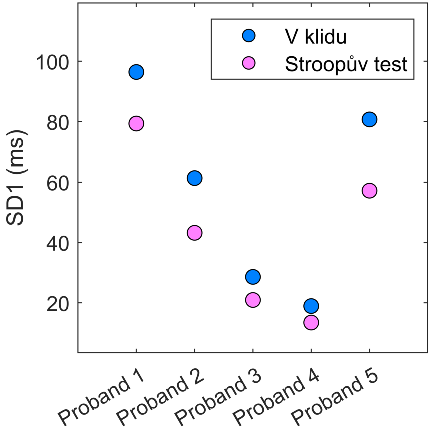
\includegraphics[width=0.9\linewidth]{../assets/figures/results_sd1}
		\caption{hodnoty SD1}
		\label{fig:results_sd1}
	\end{subfigure}
	\hfill
	\begin{subfigure}[b]{0.45\textwidth}
		\centering
		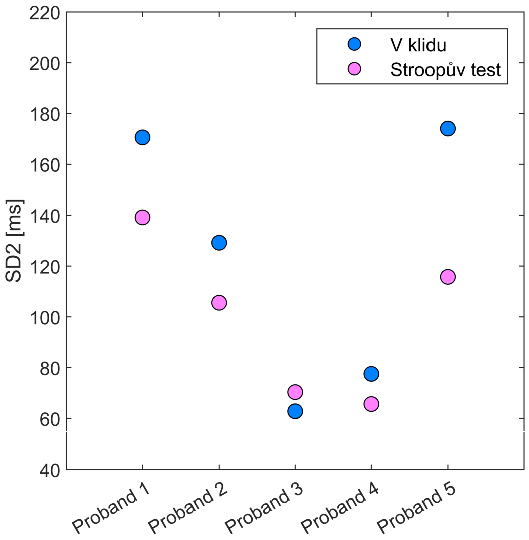
\includegraphics[width=0.9\linewidth]{../assets/figures/results_sd2}
		\caption{hodnoty SD2}
		\label{fig:results_sd2}
	\end{subfigure}
	\par\bigskip
	\begin{subfigure}[b]{0.45\textwidth}
		\centering
		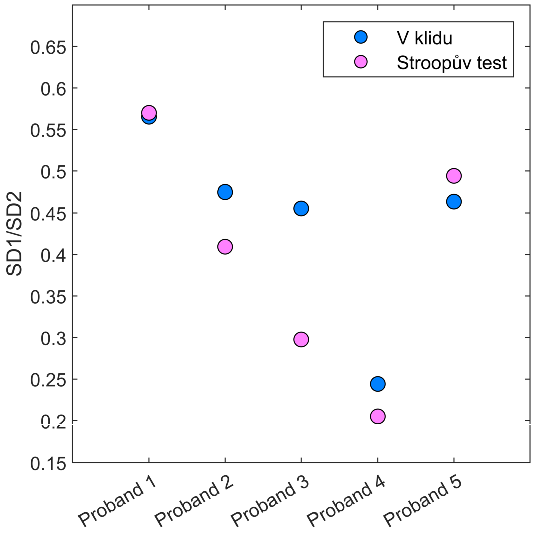
\includegraphics[width=0.9\linewidth]{../assets/figures/results_sd1sd2}
		\caption{hodnoty SD1/SD2}
		\label{fig:results_sd1sd2}
	\end{subfigure}
	\caption{Grafické porovnání sledovaných veličin v situacích N a S}
	\label{fig:results_sd_vals}
\end{figure}